\documentclass[border=3mm]{standalone}

\usepackage{tikz}
\usetikzlibrary{3d,arrows.meta}

\begin{document}
	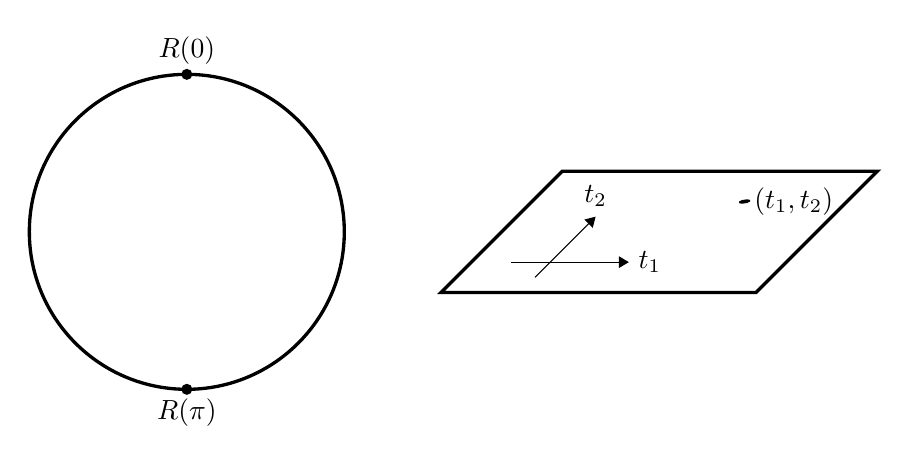
\begin{tikzpicture}
		\begin{scope}
			\draw[very thick] (0,0) circle (2cm);
			\fill (0,2) circle (2pt) node[above]{$R(0)$};
			\fill (0,-2) circle (2pt) node[below]{$R(\pi)$};
		\end{scope}
		\begin{scope}[canvas is xz plane at y=0,xshift=6cm]
			\draw[very thick] (-2,-2) rectangle (2,2);
			\draw[-Triangle] (-1,1.5) -- (-1,-0.5) node[above]{$t_2$};
			\draw[-Triangle] (-1.5,1) -- (0,1) node[right]{$t_1$};
			\fill (0.7,-1) circle (2pt) node[right]{$(t_1,t_2)$};
		\end{scope}
	\end{tikzpicture}
\end{document}